% !TEX root = ../main.tex
\chapter{Dynamikk}
\intro{Kan godt inneholde kapittel 2 og 13}

\spm{}{%
\item Hva er en kraft?
}

\newpage
\section{Krefter}
Krefter i fysikken handler rett og slett om \textit{vekselvirkning mellom legemer}. Med legemer mener vi da bestanddeler i naturen, slik som trær, mennesker, kvarker, ostehøvler, hår eller maurslukere, for å nevne noen vilkårlige eksempler. Videre i dette kapitlet skal vi studere krefter slik det defineres i fysikken. Den naturlige matematiske språkdrakten for å beskrive vekselvirkning mellom legemer er vektorer. Grunnen er at en mekanisk påkjenning vil ha både størrelse og retning.

Matematisk sett så beskrives altså krefter som vektorer. Derfor bruker vi pil over symbolet for kraft; $\vec{F},$ mens sylbolet \textit{uten} vektortegn, altså i dette tilfellet $F$, betegner størrelsen på kraften. Merk at grunnen til at vi ofte bruker bokstaven $F$ når vi prater om en kraft generelt sett er at kraft på engelsk heter \textit{force.}

La oss starte med Newton's tre kraftlover, som vi godt kan ta som selve definisjonen av hva vi mener med krefter i fysikken.
\begin{enumerate}
\item \textbf{Newtons første lov:} Dersom det ikke virker noen krefter på et legeme vil legemet forbli i ro eller fortsette med konstant fart.
\begin{align}
\Sigma\vec{F} = 0
\end{align}
\item \textbf{Newtons andre lov:} Dersom et legeme blir påvirket av én eller flere krefter vil legemet akselerere i retning av  resultant-kraften $\sum\vec{F};$
\begin{align}
\Sigma\vec{F} = m \cdot\vec{a}.
\end{align}
Her ser vi også at akselerasjonen $\vec{a}$ er en vektor, mens massen $m$ er en skalar størrelse.
\item \textbf{Newtons tredje lov:} I og med at krefter handler om \textit{vekselvirkning} mellom legemer, så optrer de \textit{alltid i par}. Mer konkret så er det slik at til enhver kraft $F$ svarer en \textit{motkraft} $F^\prime$. Disse kreftene vil være like store men motsatt rettet:

\begin{align}
\vec{F}=-\vec{F}^\prime.
\end{align}
Her brukes $(^\prime)$ bare for å signalisere at det er motkraften til $F$. Samme symbol brukes også for den deriverte, men i dette tilfelle har det ikke med derivasjon å gjøre.
\end{enumerate}
Disse tre lovene danner grunnlaget for kraftlæren slik vi fremstiller den i ingeniørfysikken.

\paragraph{Enheter:} Sånn ellers kan vi merke oss at enheten til kraft er Newton (N). Fra Newtons andre lov ser vi da at 
\[\textrm{N}=\textrm{kg}\cdot\textrm{m}/\textrm{s}^2\]



\subsection{Krefter i dagliglivet}
I dette avsnittet viser vi noen eksempler på krefter som du møter i hverdagen.

\subsubsection{Tyngdekraft}
Tyngdekraften, \textit{G}, er kraften som drar deg ned mot jorden. Jorden har en typisk tyngdeakselerasjon på 9.81 $\frac{\textrm{m}}{\textrm{s}^2}$. På månen er den 0.17 $\frac{\textrm{m}}{\textrm{s}^2}$. Denne akselerasjonen sier noe om hvor stor kraft du blir dratt ned med. Den blir skrevet som \textit{G}.
\[G=m\cdot g\]

\subsubsection{Normalkraft}
Normalkraften, \textit{N}, er kraften som gjør en motkraft på tyngdekraften. Datamaskinen som ligger på en pult står stille på pulten hvis normalkraften fra pulten er like stor som tyngdekraften. Dette samsvarer med newton's tredje lov. Normalkraften i fysikoppgavene er ofte den samme som G, bare i motsatt retning. Normalkraften kan også være lik -G$_y$, altså tyngdekraften dekomponert i y-retning. Hva \textit{N} er avhenger av det definerte koordinatsystemet og på vinkelen til bakken. 

\subsubsection{Friksjonskraft}
Friksjonskraft, \textit{R}, er krefter fra en overflate som er motsatt rettet av noe som glir langs overflaten. En ligning for friksjonskrefter, \textit{R}, står på linjen under:
\[R=\mu \cdot N\]
$\mu$ er friksjonskoeffisienten og \textit{N} er normalkraften fra bakken.
Et eksempel hvor friksjonskraft fra bakken er viktig er foreksempel på vinteren når det legger seg is på bakken. Is har lav friksjonskraft, som gjør at det er lett å skli å slå seg. Ved å strø salt eller stein på isen fører det til større friksjonskraft, og da blir det tryggere å gå på området. Et eksempel hvor det bør ha lite friksjonskraft fra bakken er en skøytebane. 

\subsubsection{Underlagskraft}
bla bla

\subsection{Dekomponering av krefter}
Figur \ref{fig:skråplankrefter1} viser en kloss som står på et skråplan. Kreftene er tegnet på. 

\begin{figure}[ht!]
    \centering
    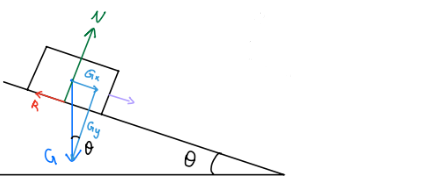
\includegraphics[width=0.7\textwidth]{Images/Kapittel3:Arbeid&Energi/Krefter i skråplan1.PNG}
    \caption{Krefter i skråplan}
    \label{fig:skråplankrefter1}
\end{figure}



\subsection{Koordinatsystem}


\exm{Kloss på skråplan}{En kloss på 3.0 kg beveger seg nedover et skråplan med en akselerasjon på 3.0 m/s. Vinkelen til skråplanet er $\theta$ 25 $^\circ$. \textbf{a)} Hva blir friksjonskrafta som virker på klossen? og \textbf{b)} Hva blir normalkraften?

Metode: \\
\textbf{a)}
Steg 1) Tegn tegning av skråplanet, klossen og kreftene som virker på klossen. Deretter dekomponer kreftene som ikke ligger parallelt med x- eller y-aksen. X- og y-aksen er tegnet høyre hjørne i Figur \ref{fig:skråplankrefter}. Kreftene som virker på boksen er normalkraften N fra bakken, tyngdekraften G, friksjonskrafta R.\\
Steg 2) Skriv opp ligninger for kreftene: \\
\[\sum\vec{F_x}=m\cdot\vec{a}\] 
\[G_x-R=m\cdot a\]   
\[R=G_x-m\cdot a\]\\  
\vspace{2pt}
For å finne G$_x$ kan det brukes trigonometri. Da kan det utledes at: \[G_x=G\cdot \sin(\theta)\]
\[G_x=m \cdot g\cdot \sin(\theta)\]
\vspace{2pt}
Da blir \textit{R}:
\[R=G_x-m\cdot a=m \cdot g\cdot \sin(\theta) -m\cdot a\]
\[R= 3\,\textrm{kg} \cdot 9.81\,\frac{\textrm{m}}{\textrm{s}^2} \cdot \sin(25^\circ) - 3\,\textrm{kg} \cdot 3\,\frac{\textrm{m}}{\textrm{s}^2}\]
\[R=-12.895\,\textrm{N}\]
\[R\approx \doubleunderline{-13\,\textrm{N}}\] \\
Det blir et negativt fortegn siden \textit{R} går i motsatt retning av definert positiv retning.
\textbf{b)}
Normalkraften virker i y-retning i koordinatsystemet. Skriver derfor opp kreftene i y-retning.
\[\sum\vec{F_y}=m\cdot\vec{a}\]\\
Akselerasjonen i y-retning er 0, siden klossen beveger seg langs x-aksen.
\[\sum\vec{F_y}=0\]
\[N-G_y=0\]
\[N=G_y\]
For å finne N trenger vi å vite G$_y$. G$_y$ kan vi finne fra de trigonometriske ligningene.
\[G_y=G\cdot \cos(\theta)\]
\[G_y=m\cdot g \cdot \cos(\theta)=3\,\textrm{kg}\cdot 9.81\,\frac{\textrm{m}}{\textrm{s}^2} \cdot \cos(25^\circ)\]
\[G_y=\doubleunderline{29.17\,\textrm{N}}\]}


\begin{figure}[ht!]
    \centering
    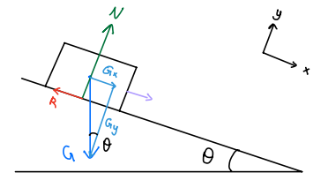
\includegraphics[width=0.6\textwidth]{Images/Kapittel3:Arbeid&Energi/Krefter i skråplan.PNG}
    \caption{Krefter i skråplan}
    \label{fig:skråplankrefter}
    \end{figure}
\newpage
\tips{Koordinatsystem}{1) Husk å definere positiv og negativ retning i koordinatsystemet. Bruk disse retningene for når du skriver ned kreftene. Går kraften i samme retning som positivt definert retning, får kraften et positivt fortegn og motsatt om kraften går i motsatt retning som den definerte positive.\\
2) Bruk de trigonometriske ligningene.}

\subsection{Krefter i sirkelbevegelse}
For sirkelbevegelse med konstant hastighet er kreftene lik:

\defn{Krefter i sirkelbevegelse}{
\[\sum \vec{F}=m\cdot \vec{a}\]
\[\sum \vec{F}=m\cdot \frac{v^2}{r}\]
}


